\documentclass[12pt,openany]{book}

\usepackage{amsmath,amssymb,amsthm}
\usepackage{graphics,epsfig,psfrag}

\topmargin          0.0in
\headheight         0.25in
\headsep            0.25in
\oddsidemargin      0.5in
\evensidemargin     0.5in
\textheight         8.5in
\textwidth          5.5in

\newtheorem{theorem}{Theorem}
\newtheorem{proposition}{Proposition}
\newtheorem{definition}{Definition}
\newtheorem{example}{Example}

\newcommand{\SetIn}{\ensuremath{\mathrm{1\!1}}}
\newcommand{\Expect}{\ensuremath{\mathrm{E}}}
\newcommand{\Var}{\ensuremath{\mathrm{Var}}}

\newcommand{\RealNumbers}{\mathbb{R}}
\newcommand{\RationalNumbers}{\mathbb{Q}}
\newcommand{\Integers}{\mathbb{Z}}
\newcommand{\NaturalNumbers}{\mathbb{N}}

%% Definitions
%%
\renewcommand{\baselinestretch}{1.25}


\begin{document}

\frontmatter

\chapter*{Copyright}
Copyright \copyright\ \\
Jean-Francois Chamberland

Permission is granted to copy, distribute and/or modify this document under the terms of the \emph{GNU Free Documentation License}, Version 1.2 or any later version published by the \emph{Free Software Foundation}; with no Invariant Sections, no Front-Cover Texts, and no Back-Cover Texts.
A copy of the license is included in the section entitled ``GNU Free Documentation License''.

\tableofcontents

\mainmatter

\chapter{Preface}

These notes provide an introduction to the fundamental concepts of digital communication systems.
The material emphasizes the unifying principles of communication theory, taking a mathematical approach to system design.
The main topics covered in these notes include sampling, quantization, data compression, channel coding, Shannon capacity and modulation theory.
Possessing some programming skills will also help in order to appreciate and use the computing material and examples contained in this document.

\section*{Major Goals}

\begin{enumerate}

\item Identify the various components of a digital communication system.
Discuss the purpose of source coding, channel coding, modulation, and equalization.
Become familiar with commonly encountered digital communication systems, and discuss how these systems can be decomposed into the same abstract constituent parts.
\item Review basic notions from Fourier analysis, including Fourier series and Fourier transforms.
Define the power spectrum of stochastic signals, and explore how it is affected by linear filtering.
\item Explore methods to convert an analog signal into a digital format through sampling and quantization.
Define the mean squared error and explain its role in assessing the performance of a digital communication system.
\item Discuss the purpose of information theory, and calculate the entropy of simple information sources.
Understand fundamental compression limits and survey efficient source coding algorithms.
\item Introduce the notions of channel capacity and error protection.
Understand how simple block codes work and compute the probability of decoding failure for simples codes.
\item Present simple modulation schemes, signal waveforms, and their vector space representations.
Characterize the structure of optimal receivers, and compute the probabilities of symbol and bit errors at the output of the demodulator.
\item Explore the properties of bandlimited channels.
Study the causes and implications of intersymbol interference, and derive the Nyquist criterion for no interference.
Review simple channel equalization schemes and go over the advantages of orthogonal frequency-division multiplexing.

\end{enumerate}


\chapter[Introduction]{Fundamentals of Statistical Signal Processing}

Statistical signal processing refers to the act of inferring generalizations from empirical data, with varying degrees of certainty.
In this introduction, we provide a unified view of detection and estimation theory.
The statistical problem we wish to explore can be described as follows.
We are interested in an unknown \emph{parameter} (or \emph{phenomenon}) which we denote by $\theta$.
We have access to an observation $Y$ that provides partial information about the value of $\theta$.
The connection between $Y$ and $\theta$ is probabilistic in nature, rather than explicit.
In particular, different values of $\theta$ may produce the same observation.
This abstract framework is illustrated below.

\begin{center}
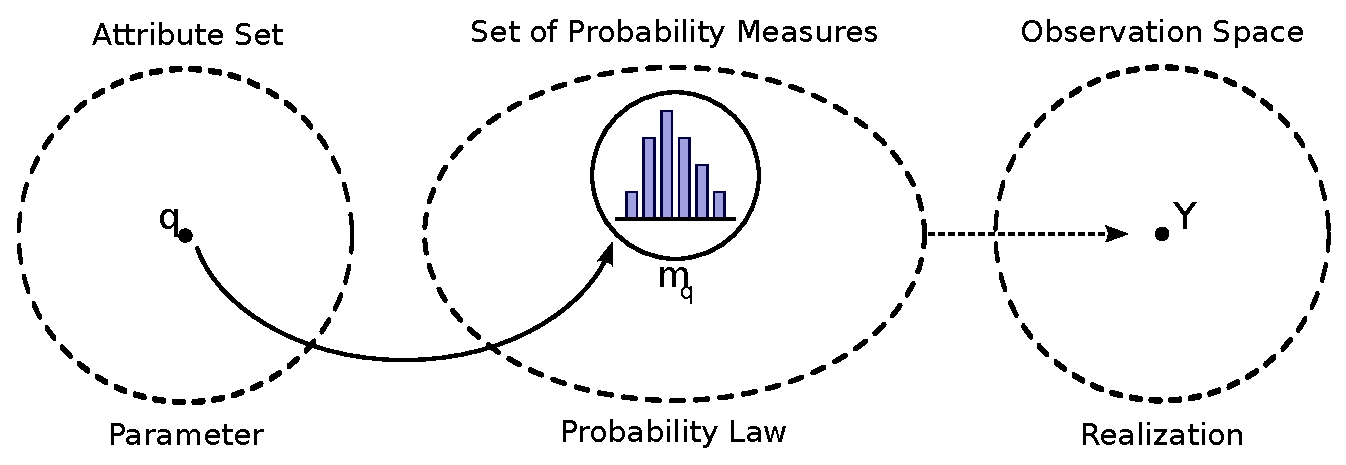
\includegraphics[width=5in]{Figures/1Chapter/Inference}
\end{center}

Three basic components are involved in this framework.
First, there is the \emph{attribute set} which is composed of all admissible values of $\theta$.
This set is represented by $U$.
The second component is a measurable space $(\mathcal{F}, \Omega)$ where $\Omega$ symbolizes the \emph{sample space} and $\mathcal{F}$ is the $\sigma$-algebra of all probability events.
Together, $\mathcal{F}$ and $\Omega$ provides a mathematical basis for the randomness induced by parameter $\theta$.
Finally, the \emph{observation space} $\Gamma$ is the collection of all realizable observations.
One obtains information about the true parameter $\theta$ by observing a random variable $Y$, which maps outcomes from the sample space $\Gamma$ to values in $\Gamma$.

If the attribute set contains a unique element, then the inference problem is trivial and we need not observe $Y$ to determine the value of $\theta$.
The more interesting case, of course, occurs when $U$ contains several distinct elements.
In this situation, the connection between $\theta$ and $Y$ becomes instrumental.
We explore this relationship next.

To each element $\theta \in U$, there corresponds a probability law $\mu_{\theta}$ acting on the measurable space $(\mathcal{F}, \Omega)$.
The true value of $\theta$ thus determines the distribution of random variable $Y$.
While observing the realization of $Y$ may provide information about its distribution, this empirical data is typically insufficient to resolve all the uncertainty surrounding the value of $\theta$.
Statistical signal processing broadly refers to the collection of techniques and methods employed to extract information about the phenomenon of interest from the available data.

\begin{center}
\includegraphics[width=3in]{Figures/1Chapter/StatisticalSignalProcessing}
\end{center}

We provide a simple example below to illustrate how this framework applies to engineering problems.

\begin{example} \label{example:BinaryCommunicationSystem}
A digital communication system transmits a single bit over a noisy channel, using a zero or a one.
The received information is corrupted by additive Gaussian noise, with distribution $\mathcal{N}(0,1)$.
We wish to decide which bit was sent from the received information.
To initiate this process, we cast this problem in the abstract framework described above.
In the present case, the attribute set is $U = \{ 0, 1 \}$; the sample space is the real line; and the corresponding probability density functions are
\begin{equation*}
f_0 (y) = \frac{1}{\sqrt{2 \pi}} e^{- \frac{y^2}{2}} \quad
f_1 (y) = \frac{1}{\sqrt{2 \pi}} e^{- \frac{(y-1)^2}{2}} .
\end{equation*}
Note that in this first example the observation space and the sample space are identical.
\end{example}

The primary characteristics that distinguish statistical inference problems from one another are the amount of a priori knowledge available about the attribute set $U$, the goal underlying the inference procedure, and the performance criterion used to assess the effectiveness of the inference procedure.
If the attribute set is partitioned into a finite or countable number of subsets and the objective is to identify which subset $\theta$ belongs to, then the decision process is termed \emph{detection} or \emph{hypothesis testing}.
In particular, a detector maps every element in the observation space $\Gamma$ to one of the admissible hypotheses.
A graphical interpretation of a detection process is illustrated below.

\begin{center}
\includegraphics[width=3in]{Figures/1Chapter/DetectionModel}
\end{center}

On the other hand, if $U$ contains an uncountable number of candidates and we are tasked with selecting the most appropriate one, then we are facing an \emph{estimation} problem.
In this setting, the goal is to select an estimate $\hat{\theta}$ based on observation $Y$ as to optimize a given objective function.
Thus, parameter estimation is a procedure that takes an argument in observation space $\Gamma$ and returns an element in the attribute set $U$.
The distinction between detection and estimation is at times rhetorical;
we will not delve on this issue.
Rather, our focus will be to develop a solid understanding of statistical signal processing and to become well-versed in applying some of its techniques and algorithms.

A second important distinction among inference problems, as mentioned above, comes from the assumptions made on attribute set $U$.
In \emph{classical estimation}, $U$ is taken to be a specific set containing the unknown parameter $\theta$.
This can be contrasted with the \emph{Bayesian approach} where $U$ is assumed to be a probability space with a specific distribution.
In this latter case, the value of $\theta$ is itself the outcome of a random experiment.
The distinction between these two approaches leads to disparate performance criteria, and hence different estimators.
Such a distinction is also present in detection problems, where the attribute set is either a collection of object with a deterministic parameter $\theta$, or a measurable space with a certain probability law.

A final and less straightforward distinction between inference problems stems from the nature of the empirical observations.
The framework detailed above implicitly assumes that observations can be viewed as random variables.
If on the other hand we have access to empirical data coming from a random process, then the inference problem becomes more challenging.
In this scenario, inference problems are referred to as \emph{signal detection} and \emph{signal estimation}.
When dealing with the progressive estimation of a stochastic process, the statistical inference procedure is often called \emph{filtering}.
We will address some of these problems once we acquire the mathematical sophistication necessary to tackle them.


\section{Modeling Engineering Problems}

These notes present a collection of important tools and methods in statistical signal processing.
Becoming familiar with these tools should provide the reader with the ability to solve various inference problems, and to assess the performance of the corresponding statistical procedures.
Still, an equally important skill to develop is the capacity to take a concrete engineering problem and to formulate it mathematically in a way that leads to a meaningful solution.
In this exposition, we will often use an abstract problem formulation as our starting point.
However, the value of being able to take an engineering challenge and to cast it in a relevant yet solvable framework is not to be understated.
Developing this skill is partly what sets apart the value of one's education and experience.
Throughout, we will provide examples and case studies of meaningful problems together with suitable mathematical interpretations.
Reading there examples carefully and understanding the process of selecting the proper tools to solve them should help develop good intuition.
While going through these notes, one should also try to think about new situations where the statistical methods under consideration apply.



%\section{Organization}
%
%These notes are organized as follows.
%
%In Chapter~\ref{chapter:Detection}, we study hypothesis testing.
%We begin with an introduction to the simplest such problem, binary detection.
%Both the classical and Bayesian forms of the problem are considered.
%The theory of detection is then extended to composite hypothesis testing, a framework where the attribute set contains more than two elements.
%We also discuss the problem of robust detection, sequential detection and quickest change detection.
%Finally, we look at simple instances of $M$-ary hypothesis testing.

%Chapter~\ref{chapter:ClassicalParameterEstimation} is devoted to classical parameter estimation.
%We first introduce the celebrated Cramer-Rao lower bound, which provides a performance limit on unbiased estimators.
%We then present the concept of sufficient statistics.
%This is followed by a discussion of common estimators including the best linear unbiased estimator, the maximum likelihood estimator, and the least squares estimator.
%The expectation-maximization algorithm is also introduced as a numerically tractable estimation methodology.
%
%Chapter~\ref{chapter:BayesianParameterEstimation} presents a study of Bayesian parameter estimation.
%The maximum a posteriori estimator is first introduced.
%This is followed by a discussion of the minimum mean square error and linear minimum mean square error estimators.
%Signal estimation is treated in Chapter~\ref{chapter:SignalEstimation}, where the Kalman-Bucy filter and the Wiener-Kolmogorov filter are introduced.

%estimating the median of a number of integers to which you only have a few observations.





%\appendix

%\chapter{GNU Free Documentation License}

\begin{center}
Version 1.2, November 2002 \\
Copyright \copyright 2000, 2001, 2002 \\
Free Software Foundation, Inc. \\
51 Franklin St, Fifth Floor \\
Boston, MA 02110-1301 \\
USA

Everyone is permitted to copy and distribute verbatim copies
of this license document, but changing it is not allowed.
\end{center}

\section{Preamble}

The purpose of this License is to make a manual, textbook, or other functional and useful document ``free'' in the sense of freedom:
to assure everyone the effective freedom to copy and redistribute it, with or without modifying it, either commercially or noncommercially.
Secondarily, this License preserves for the author and publisher a way to get credit for their work, while not being considered responsible for modifications made by others.

This License is a kind of ``copyleft'', which means that derivative works of the document must themselves be free in the same sense.
It complements the GNU General Public License, which is a copyleft license designed for free software.

We have designed this License in order to use it for manuals for free software, because free software needs free documentation:
a free program should come with manuals providing the same freedoms that the software does.
But this License is not limited to software manuals; it can be used for any textual work, regardless of subject matter or whether it is published as a printed book.
We recommend this License principally for works whose purpose is instruction or reference.


\section{Applicability and Definitions}

This License applies to any manual or other work, in any medium, that contains a notice placed by the copyright holder saying it can be distributed under the terms of this License.
Such a notice grants a world-wide, royalty-free license, unlimited in duration, to use that work under the conditions stated herein.  The \textbf{``Document''}, below, refers to any such manual or work.
Any member of the public is a licensee, and is addressed as \textbf{``you''}.
You accept the license if you copy, modify or distribute the work in a way requiring permission under copyright law.

A \textbf{``Modified Version''} of the Document means any work containing the
Document or a portion of it, either copied verbatim, or with
modifications and/or translated into another language.

A \textbf{``Secondary Section''} is a named appendix or a front-matter section of
the Document that deals exclusively with the relationship of the
publishers or authors of the Document to the Document's overall subject
(or to related matters) and contains nothing that could fall directly
within that overall subject.  (Thus, if the Document is in part a
textbook of mathematics, a Secondary Section may not explain any
mathematics.)  The relationship could be a matter of historical
connection with the subject or with related matters, or of legal,
commercial, philosophical, ethical or political position regarding
them.

The \textbf{``Invariant Sections''} are certain Secondary Sections whose titles
are designated, as being those of Invariant Sections, in the notice
that says that the Document is released under this License.  If a
section does not fit the above definition of Secondary then it is not
allowed to be designated as Invariant.  The Document may contain zero
Invariant Sections.  If the Document does not identify any Invariant
Sections then there are none.

The \textbf{``Cover Texts''} are certain short passages of text that are listed,
as Front-Cover Texts or Back-Cover Texts, in the notice that says that
the Document is released under this License.  A Front-Cover Text may
be at most 5 words, and a Back-Cover Text may be at most 25 words.

A \textbf{``Transparent''} copy of the Document means a machine-readable copy,
represented in a format whose specification is available to the
general public, that is suitable for revising the document
straightforwardly with generic text editors or (for images composed of
pixels) generic paint programs or (for drawings) some widely available
drawing editor, and that is suitable for input to text formatters or
for automatic translation to a variety of formats suitable for input
to text formatters.  A copy made in an otherwise Transparent file
format whose markup, or absence of markup, has been arranged to thwart
or discourage subsequent modification by readers is not Transparent.
An image format is not Transparent if used for any substantial amount
of text.  A copy that is not ``Transparent'' is called \textbf{``Opaque''}.

Examples of suitable formats for Transparent copies include plain
ASCII without markup, Texinfo input format, LaTeX input format, SGML
or XML using a publicly available DTD, and standard-conforming simple
HTML, PostScript or PDF designed for human modification.  Examples of
transparent image formats include PNG, XCF and JPG.  Opaque formats
include proprietary formats that can be read and edited only by
proprietary word processors, SGML or XML for which the DTD and/or
processing tools are not generally available, and the
machine-generated HTML, PostScript or PDF produced by some word
processors for output purposes only.

The \textbf{``Title Page''} means, for a printed book, the title page itself,
plus such following pages as are needed to hold, legibly, the material
this License requires to appear in the title page.  For works in
formats which do not have any title page as such, ``Title Page'' means
the text near the most prominent appearance of the work's title,
preceding the beginning of the body of the text.

A section \textbf{``Entitled XYZ''} means a named subunit of the Document whose
title either is precisely XYZ or contains XYZ in parentheses following
text that translates XYZ in another language.  (Here XYZ stands for a
specific section name mentioned below, such as \textbf{``Acknowledgements''},
\textbf{``Dedications''}, \textbf{``Endorsements''}, or \textbf{``History''}.)  
To \textbf{``Preserve the Title''}
of such a section when you modify the Document means that it remains a
section ``Entitled XYZ'' according to this definition.

The Document may include Warranty Disclaimers next to the notice which
states that this License applies to the Document.  These Warranty
Disclaimers are considered to be included by reference in this
License, but only as regards disclaiming warranties: any other
implication that these Warranty Disclaimers may have is void and has
no effect on the meaning of this License.


\section{Verbatim Copying}

You may copy and distribute the Document in any medium, either
commercially or noncommercially, provided that this License, the
copyright notices, and the license notice saying this License applies
to the Document are reproduced in all copies, and that you add no other
conditions whatsoever to those of this License.  You may not use
technical measures to obstruct or control the reading or further
copying of the copies you make or distribute.  However, you may accept
compensation in exchange for copies.  If you distribute a large enough
number of copies you must also follow the conditions in section 3.

You may also lend copies, under the same conditions stated above, and
you may publicly display copies.


\section{Copying in Quantity}

If you publish printed copies (or copies in media that commonly have
printed covers) of the Document, numbering more than 100, and the
Document's license notice requires Cover Texts, you must enclose the
copies in covers that carry, clearly and legibly, all these Cover
Texts: Front-Cover Texts on the front cover, and Back-Cover Texts on
the back cover.  Both covers must also clearly and legibly identify
you as the publisher of these copies.  The front cover must present
the full title with all words of the title equally prominent and
visible.  You may add other material on the covers in addition.
Copying with changes limited to the covers, as long as they preserve
the title of the Document and satisfy these conditions, can be treated
as verbatim copying in other respects.

If the required texts for either cover are too voluminous to fit
legibly, you should put the first ones listed (as many as fit
reasonably) on the actual cover, and continue the rest onto adjacent
pages.

If you publish or distribute Opaque copies of the Document numbering
more than 100, you must either include a machine-readable Transparent
copy along with each Opaque copy, or state in or with each Opaque copy
a computer-network location from which the general network-using
public has access to download using public-standard network protocols
a complete Transparent copy of the Document, free of added material.
If you use the latter option, you must take reasonably prudent steps,
when you begin distribution of Opaque copies in quantity, to ensure
that this Transparent copy will remain thus accessible at the stated
location until at least one year after the last time you distribute an
Opaque copy (directly or through your agents or retailers) of that
edition to the public.

It is requested, but not required, that you contact the authors of the
Document well before redistributing any large number of copies, to give
them a chance to provide you with an updated version of the Document.


\section{Modifications}

You may copy and distribute a Modified Version of the Document under
the conditions of sections 2 and 3 above, provided that you release
the Modified Version under precisely this License, with the Modified
Version filling the role of the Document, thus licensing distribution
and modification of the Modified Version to whoever possesses a copy
of it.  In addition, you must do these things in the Modified Version:

\begin{itemize}
\item[A.] 
   Use in the Title Page (and on the covers, if any) a title distinct
   from that of the Document, and from those of previous versions
   (which should, if there were any, be listed in the History section
   of the Document).  You may use the same title as a previous version
   if the original publisher of that version gives permission.
   
\item[B.]
   List on the Title Page, as authors, one or more persons or entities
   responsible for authorship of the modifications in the Modified
   Version, together with at least five of the principal authors of the
   Document (all of its principal authors, if it has fewer than five),
   unless they release you from this requirement.
   
\item[C.]
   State on the Title page the name of the publisher of the
   Modified Version, as the publisher.
   
\item[D.]
   Preserve all the copyright notices of the Document.
   
\item[E.]
   Add an appropriate copyright notice for your modifications
   adjacent to the other copyright notices.
   
\item[F.]
   Include, immediately after the copyright notices, a license notice
   giving the public permission to use the Modified Version under the
   terms of this License, in the form shown in the Addendum below.
   
\item[G.]
   Preserve in that license notice the full lists of Invariant Sections
   and required Cover Texts given in the Document's license notice.
   
\item[H.]
   Include an unaltered copy of this License.
   
\item[I.]
   Preserve the section Entitled ``History'', Preserve its Title, and add
   to it an item stating at least the title, year, new authors, and
   publisher of the Modified Version as given on the Title Page.  If
   there is no section Entitled ``History'' in the Document, create one
   stating the title, year, authors, and publisher of the Document as
   given on its Title Page, then add an item describing the Modified
   Version as stated in the previous sentence.
   
\item[J.]
   Preserve the network location, if any, given in the Document for
   public access to a Transparent copy of the Document, and likewise
   the network locations given in the Document for previous versions
   it was based on.  These may be placed in the ``History'' section.
   You may omit a network location for a work that was published at
   least four years before the Document itself, or if the original
   publisher of the version it refers to gives permission.
   
\item[K.]
   For any section Entitled ``Acknowledgements'' or ``Dedications'',
   Preserve the Title of the section, and preserve in the section all
   the substance and tone of each of the contributor acknowledgements
   and/or dedications given therein.
   
\item[L.]
   Preserve all the Invariant Sections of the Document,
   unaltered in their text and in their titles.  Section numbers
   or the equivalent are not considered part of the section titles.
   
\item[M.]
   Delete any section Entitled ``Endorsements''.  Such a section
   may not be included in the Modified Version.
   
\item[N.]
   Do not retitle any existing section to be Entitled ``Endorsements''
   or to conflict in title with any Invariant Section.
   
\item[O.]
   Preserve any Warranty Disclaimers.
\end{itemize}

If the Modified Version includes new front-matter sections or
appendices that qualify as Secondary Sections and contain no material
copied from the Document, you may at your option designate some or all
of these sections as invariant.  To do this, add their titles to the
list of Invariant Sections in the Modified Version's license notice.
These titles must be distinct from any other section titles.

You may add a section Entitled ``Endorsements'', provided it contains
nothing but endorsements of your Modified Version by various
parties--for example, statements of peer review or that the text has
been approved by an organization as the authoritative definition of a
standard.

You may add a passage of up to five words as a Front-Cover Text, and a
passage of up to 25 words as a Back-Cover Text, to the end of the list
of Cover Texts in the Modified Version.  Only one passage of
Front-Cover Text and one of Back-Cover Text may be added by (or
through arrangements made by) any one entity.  If the Document already
includes a cover text for the same cover, previously added by you or
by arrangement made by the same entity you are acting on behalf of,
you may not add another; but you may replace the old one, on explicit
permission from the previous publisher that added the old one.

The author(s) and publisher(s) of the Document do not by this License
give permission to use their names for publicity for or to assert or
imply endorsement of any Modified Version.


\section{Combining Documents}

You may combine the Document with other documents released under this
License, under the terms defined in section 4 above for modified
versions, provided that you include in the combination all of the
Invariant Sections of all of the original documents, unmodified, and
list them all as Invariant Sections of your combined work in its
license notice, and that you preserve all their Warranty Disclaimers.

The combined work need only contain one copy of this License, and
multiple identical Invariant Sections may be replaced with a single
copy.  If there are multiple Invariant Sections with the same name but
different contents, make the title of each such section unique by
adding at the end of it, in parentheses, the name of the original
author or publisher of that section if known, or else a unique number.
Make the same adjustment to the section titles in the list of
Invariant Sections in the license notice of the combined work.

In the combination, you must combine any sections Entitled ``History''
in the various original documents, forming one section Entitled
``History''; likewise combine any sections Entitled ``Acknowledgements'',
and any sections Entitled ``Dedications''.  You must delete all sections
Entitled ``Endorsements''.


\section{Collections of Documents}

You may make a collection consisting of the Document and other documents
released under this License, and replace the individual copies of this
License in the various documents with a single copy that is included in
the collection, provided that you follow the rules of this License for
verbatim copying of each of the documents in all other respects.

You may extract a single document from such a collection, and distribute
it individually under this License, provided you insert a copy of this
License into the extracted document, and follow this License in all
other respects regarding verbatim copying of that document.


\section{Aggregation with Independent Works}

A compilation of the Document or its derivatives with other separate
and independent documents or works, in or on a volume of a storage or
distribution medium, is called an ``aggregate'' if the copyright
resulting from the compilation is not used to limit the legal rights
of the compilation's users beyond what the individual works permit.
When the Document is included in an aggregate, this License does not
apply to the other works in the aggregate which are not themselves
derivative works of the Document.

If the Cover Text requirement of section 3 is applicable to these
copies of the Document, then if the Document is less than one half of
the entire aggregate, the Document's Cover Texts may be placed on
covers that bracket the Document within the aggregate, or the
electronic equivalent of covers if the Document is in electronic form.
Otherwise they must appear on printed covers that bracket the whole
aggregate.


\section{Translation}

Translation is considered a kind of modification, so you may
distribute translations of the Document under the terms of section 4.
Replacing Invariant Sections with translations requires special
permission from their copyright holders, but you may include
translations of some or all Invariant Sections in addition to the
original versions of these Invariant Sections.  You may include a
translation of this License, and all the license notices in the
Document, and any Warranty Disclaimers, provided that you also include
the original English version of this License and the original versions
of those notices and disclaimers.  In case of a disagreement between
the translation and the original version of this License or a notice
or disclaimer, the original version will prevail.

If a section in the Document is Entitled ``Acknowledgements'',
``Dedications'', or ``History'', the requirement (section 4) to Preserve
its Title (section 1) will typically require changing the actual
title.


\section{Termination}

You may not copy, modify, sublicense, or distribute the Document except
as expressly provided for under this License.  Any other attempt to
copy, modify, sublicense or distribute the Document is void, and will
automatically terminate your rights under this License.  However,
parties who have received copies, or rights, from you under this
License will not have their licenses terminated so long as such
parties remain in full compliance.


\section{Future Revisions of this License}

The Free Software Foundation may publish new, revised versions
of the GNU Free Documentation License from time to time.  Such new
versions will be similar in spirit to the present version, but may
differ in detail to address new problems or concerns.  See
http://www.gnu.org/copyleft/.

Each version of the License is given a distinguishing version number.
If the Document specifies that a particular numbered version of this
License ``or any later version'' applies to it, you have the option of
following the terms and conditions either of that specified version or
of any later version that has been published (not as a draft) by the
Free Software Foundation.  If the Document does not specify a version
number of this License, you may choose any version ever published (not
as a draft) by the Free Software Foundation.

\end{document}
